% CS F407 Artificial Intelligence: final project report template.
% Limit: 2 pages, including everything except references.
% Do not change the font size, margins or spacing.
\documentclass[11pt,a4paper,twocolumn]{article}

\usepackage[margin=2cm,columnsep=0.8cm]{geometry}
\usepackage[T1]{fontenc}
\usepackage{lmodern}
\usepackage{microtype}
\usepackage{amsmath,amssymb}
\usepackage{graphicx}
\usepackage{booktabs}
\usepackage{tabularx}
\usepackage{enumitem}
\usepackage{titlesec}
\usepackage[hidelinks]{hyperref}

\titleformat{\section}{\normalsize\bfseries}{\thesection}{0.6em}{}
\titlespacing*{\section}{0pt}{1.2ex plus 0.3ex}{0.6ex}
\setlist{nosep,leftmargin=*}
\setlength{\parskip}{0.3ex}

\newcommand{\coursename}{CS F407 Artificial Intelligence, AY 2026--27 Semester I}
\newcommand{\teamno}{Team: The Unsupervised}
\newcommand{\githuburl}{https://github.com/AdityaKalra2410/next-ravi-varma}

\begin{document}

\twocolumn[{%
\begin{center}
  {\large\bfseries The Next Ravi Varma: Generating Epic Scenes in Raja Ravi Varma's Oil-Painting Style with a Style LoRA, LLM Prompt Expansion and Pose Control}\\[1ex]
  \teamno\\
  Aditya Kalra (2024A7PS0536G), Eshan Singhai (2024ADPS0836G), Rishit Khanna (2024A3PS0343G), Mayank Bhojwani (2024A7PS0639G)\\[0.5ex]
  {\small \coursename, BITS Pilani, K.K. Birla Goa Campus}\\[1.5ex]
  \begin{minipage}{0.85\textwidth}
    \small
    \centerline{\bfseries Abstract}\vspace{0.5ex}
    Raja Ravi Varma (1848--1906) painted scenes from the Indian epics in a European academic oil style,
    but general text-to-image models reproduce the flat look of the cheap prints of his work instead.
    We build a system that turns a short scene description, and optionally a photo of a pose, into a new
    painting in his oil style. We curate 61 oil paintings, caption them with an open vision-language model,
    train a rank-4 LoRA on Stable Diffusion~1.5, add LLM prompt expansion with CLIP-based best-of-4
    selection, and add ControlNet (OpenPose) so figures follow a pose photo. On held-out evaluations
    with CLIP ViT-L/14, the LoRA raises style similarity to unseen Varma paintings from 0.731 to 0.816
    (real paintings: 0.839), best-of-4 selection raises scene match from 28.2 to 30.4, and ControlNet raises
    pose accuracy (PCK@0.1) from 0.10 to 0.97 at a small style cost (0.834 to 0.815). A Gradio web app
    exposes the full pipeline.
  \end{minipage}
\end{center}
\vspace{1.5ex}
}]

\section{Introduction}
Inspired by ``The Next Rembrandt''~\cite{nextrembrandt}, we ask whether a small, curated corpus is enough
to teach a diffusion model the style of Raja Ravi Varma, whose paintings defined the visual image of the
Mahabharata and Ramayana. The difficulty is that his style is known online mostly through oleographs
(chromolithograph prints from his press) and calendar art, so prompting a base model with his name gives
bright, flat images rather than his blended oil rendering and chiaroscuro.

\textbf{Input:} an English scene description (e.g.\ ``Hanuman kneeling in devotion''), optionally a photo
of a person posing. \textbf{Output:} a new painting of that scene in Varma's oil style whose figure follows
the pose. \textbf{Contributions:} (i)~a curated, captioned dataset of his oil paintings with a held-out test
set; (ii)~a style LoRA; (iii)~an LLM prompt-expansion and best-of-$N$ selection module; (iv)~pose control with
ControlNet, a character-appearance table and pose-aware selection; (v)~quantitative evaluations of each stage
and a web app.

\section{Background and related work}
Latent diffusion models~\cite{ho2020ddpm,rombach2022ldm} generate images by iteratively denoising a latent
conditioned on a CLIP text embedding. LoRA~\cite{hu2022lora} adapts a frozen network by learning a low-rank
update to its weight matrices; together with a rare trigger phrase in the captions (as in
DreamBooth~\cite{ruiz2023dreambooth}) it lets a style be learned from tens of images. ControlNet~\cite{zhang2023controlnet}
adds a trainable copy of the encoder that injects a spatial condition, here an OpenPose~\cite{cao2021openpose}
skeleton. CLIP~\cite{radford2021clip} gives a shared image--text embedding that we use both to select and,
with a different model, to evaluate images, following CLIPScore~\cite{hessel2021clipscore}. Captions come from
vision-language models (BLIP-2~\cite{li2023blip2}, LLaVA~\cite{liu2023llava}, Qwen3-VL~\cite{qwen3vl}); prompt
expansion uses Qwen2.5~\cite{qwen25}. Pose accuracy is measured with PCK~\cite{yang2013pck}.

\section{Method}
\textbf{Dataset (M1).} We downloaded 135 images from the Wikimedia Commons category of Varma's paintings
(public domain; shorter side $\geq$768\,px). Near-duplicate scans were grouped with a 64-bit perceptual hash
(Hamming distance $\leq 8$) and checked by hand; 38 duplicates and 4 non-Varma items were removed. Each
remaining image was labelled oil or oleograph from Commons titles and visual cues (flat colour, hard outlines
and printed borders vs.\ blended shading and canvas texture). We keep only the \textbf{61 oil paintings} and
split them into 52 training and 9 test paintings that are never used for training or for selecting outputs.

\textbf{Captions.} Each painting gets a 10-field tag template (figures, characters, attire, pose, action,
setting, composition, mood, lighting, palette). BLIP-2 produced generic one-liners; LLaVA-1.5/1.6-7B looped
and invented characters from the painting's title. Qwen3-VL-8B (4-bit) returned valid tags for all 61.
Training captions use only the seven content fields, prefixed by the trigger phrase
\texttt{rrvarma oil painting} and trimmed to CLIP's 77 tokens from the end. Style words are never in the
captions, so the style can only attach to the trigger.

\textbf{Style LoRA (M2).} Stable Diffusion~1.5 stays frozen. For each attention projection
$W\in\mathbb{R}^{d\times k}$ of the UNet (query, key, value, output of self- and cross-attention) we learn
$W' = W + BA$ with $A\in\mathbb{R}^{r\times k}$, $B\in\mathbb{R}^{d\times r}$, $r=4$ and $B$ initialised to
zero (${\approx}0.8$M parameters, 3\,MB). Training minimises the standard denoising loss
$\mathbb{E}_{z_0,\epsilon,t}\,\lVert \epsilon - \epsilon_\theta(z_t, t, c)\rVert^2$ over (image, caption)
pairs; since the trigger is the only text shared by all captions and the style is the only visual feature
shared by all images, the trigger absorbs the style.

\textbf{Prompt expansion and selection (M3).} Qwen2.5-7B-Instruct (4-bit) is prompted with a system message
and two worked examples to fill a JSON object with the same fields as our training tags. Code then repairs
the output: it keeps every capitalised name from the user's text, moves place names to the setting, makes
the composition agree with the number of figures, removes style words and trims to 77 tokens. A
\emph{hybrid} mode keeps the user's sentence and appends figures, pose, setting and composition. For
selection we generate $N{=}4$ candidates and keep the one maximising
$\cos(f(x), g(\text{scene})) + \cos(f(x), \bar{f}_{\text{train}})$, where $f,g$ are CLIP ViT-B/32 image and
text encoders and $\bar{f}_{\text{train}}$ is the mean embedding of the 52 \emph{training} paintings. A
negative prompt (``calendar art, poster, flat colors, oversaturated, cartoon, photograph, \ldots'') steers
away from the print look.

\textbf{Pose control (M4).} OpenPose extracts a body skeleton from the user's photo; only the skeleton is
passed to ControlNet (\texttt{control\_v11p\_sd15\_openpose}), which shares the LoRA-adapted UNet, so the
photo's colours and clothes cannot leak into the painting. Because SD~1.5 does not know what most epic
characters look like (it painted Bharata as an old sage and Arjuna as a woman), a table of 31 characters
appends gender, age and traditional attire for the characters named in the scene (only for as many as there
are people in the skeleton). Best-of-4 becomes pose-aware: OpenPose is run again on every candidate, those
whose pose accuracy is more than 0.15 below the best are dropped, then the CLIP score above decides.
Finally a high-resolution refinement (SDEdit-style img2img~\cite{meng2022sdedit}) upscales the chosen image
$1.5\times$ and re-noises it to strength 0.35, which keeps the layout but redraws faces and hands that are
only ${\sim}40$\,px tall at 512\,px.

\begin{figure*}[t]
  \centering
  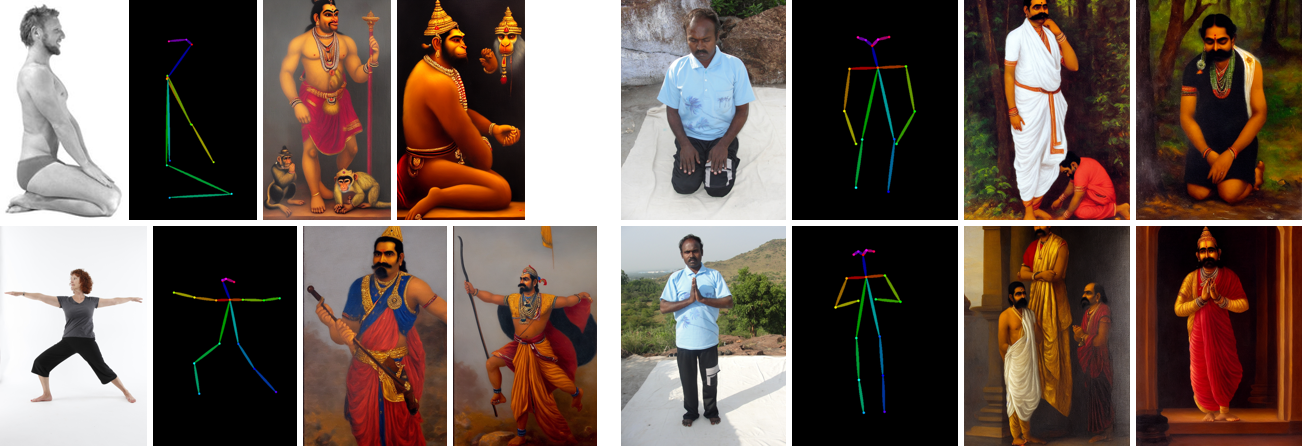
\includegraphics[width=\textwidth]{fig_m4.png}
  \caption{M4 examples from the evaluation (seed 0, no hand-picking). Each strip: pose photo, extracted
  skeleton, painting \emph{without} ControlNet, painting \emph{with} ControlNet (final pipeline). Scenes:
  Hanuman kneeling, Bharata kneeling in the forest (top); Bhima in a battle stance, Vibhishana with folded
  hands (bottom). Without ControlNet the text alone fails to produce kneeling, the stance or the folded hands,
  and extra figures appear.}
  \label{fig:m4}
\end{figure*}

\section{Experimental setup}
All experiments ran on a free Google Colab T4 GPU (fp16, DPM-Solver, 30 steps, guidance 7.5) with
\texttt{diffusers}, \texttt{transformers}, \texttt{peft} and \texttt{controlnet\_aux}. The evaluator is
CLIP ViT-L/14, deliberately different from the ViT-B/32 used for selection. \textbf{Scene/prompt match} is
$100\cdot\cos$ between the image and the user's original text. \textbf{Style} is the cosine similarity to the
mean embedding of the 9 held-out test paintings; the test paintings themselves score 0.839 against their own
mean (a slightly generous ceiling). \textbf{Pose accuracy} is PCK@0.1: OpenPose is run on the painting and we
count the fraction of the photo's detected joints that lie within $0.1\times$ the body's bounding-box size of
the same joint.
\textbf{M2:} 10 new epic prompts $\times$ 2 seeds, comparing base SD, base SD with
``in the style of Raja Ravi Varma, oil painting'', and SD with our LoRA; we also check memorisation (maximum
similarity to any training image) and reconstruct the 9 test paintings from their own captions.
\textbf{M3:} 10 short scenes $\times$ 2 seeds, six prompt/selection variants.
\textbf{M4:} 8 single-person pose photos from Wikimedia Commons (kneeling, archery, warrior stance,
meditation, folded hands, arms raised), each paired with an epic scene, $\times$ 2 seeds. The three
conditions share the prompt, negative prompt, image size, best-of-4 and refinement and differ only in
ControlNet and the selection rule; both ControlNet conditions select from the same four candidates.

\section{Results}
\begin{table}[h]
\centering
\small
\begin{tabular}{lcc}
\toprule
M2: condition & Prompt match & Style \\
\midrule
Base SD 1.5 & 28.36 & 0.731 \\
+ ``style of Ravi Varma'' & 25.57 & 0.790 \\
\textbf{SD 1.5 + our LoRA} & \textbf{29.37} & \textbf{0.816} \\
\midrule
Real test paintings & -- & 0.839 \\
\bottomrule
\end{tabular}
\caption{Style LoRA (20 images per row). Higher is better for both.}
\label{tab:m2}
\end{table}

\textbf{Style (Table~\ref{tab:m2}).} The LoRA closes about 80\% of the style gap between base SD and real
paintings and gives the best style score on 9 of 10 prompts, while also improving prompt match. Naming the
artist raises style only to 0.790 and hurts prompt match: visually it produces bright calendar-print art,
the look we excluded. No output is a copy of a training painting (maximum similarity 0.897, below a 0.95
threshold). In reconstruction, CLIP identifies the correct test painting from the LoRA's output 15/18 times
(base SD 12/18, chance 2/18).

\begin{table}[h]
\centering
\small
\begin{tabular}{lcc}
\toprule
M3: prompt / selection & Scene & Style \\
\midrule
raw \texttt{trigger, scene} & 28.20 & 0.823 \\
full LLM expansion & 27.28 & 0.811 \\
hybrid expansion & 28.71 & 0.815 \\
hybrid + neg.\ prompt & 27.67 & 0.817 \\
\textbf{raw + neg.\ + best-of-4} & \textbf{30.40} & \textbf{0.831} \\
hybrid + neg.\ + best-of-4 & 29.17 & 0.824 \\
\bottomrule
\end{tabular}
\caption{Prompt expansion and selection (20 images per row).}
\label{tab:m3}
\end{table}

\textbf{Prompt expansion (Table~\ref{tab:m3}).} Best-of-4 selection gives the largest gain (+2.2 scene match,
+0.008 style) and is best on 6 of 10 scenes. LLM expansion does not raise CLIP scores for full-sentence inputs;
visually it helps include missing characters and helps very short inputs, so it is an option rather than the
default.

\begin{table}[h]
\centering
\small
\setlength{\tabcolsep}{4pt}
\begin{tabular}{lccc}
\toprule
M4: condition & Pose & Scene & Style \\
\midrule
no ControlNet & 0.097 & 28.22 & \textbf{0.834} \\
ControlNet + CLIP pick & 0.962 & 28.27 & 0.814 \\
\textbf{+ pose-aware pick} &\textbf{0.969} & \textbf{28.57} & 0.815 \\
\bottomrule
\end{tabular}
\caption{Pose control (8 poses $\times$ 2 seeds = 16 images per row). Pose = PCK@0.1, higher is better.
A person was detected in 100\% of paintings in every condition.}
\label{tab:m4}
\end{table}

\textbf{Pose control (Table~\ref{tab:m4}, Fig.~\ref{fig:m4}).} From text alone, only 10\% of the photo's
joints land in the right place; with ControlNet, 96--97\% do, with no loss in scene match. Style drops by
0.02 because a forced pose moves the image away from Varma's usual compositions, but it remains far above
base SD (0.731). Pose-aware selection adds only a small gain, since ControlNet's candidates are already
almost all correct.

\section{Discussion and limitations}
Each stage improves its target metric: the LoRA transfers the oil style from 52 images, best-of-$N$ selection
improves scene match, and ControlNet solves the poses that text conditioning cannot (kneeling, drawing a bow,
folded hands). Limitations: (i)~the corpus is small and dominated by single-woman portraits, so male
characters can drift feminine and many outputs share a warm amber/red cast; the character table mitigates
but does not remove this. (ii)~SD~1.5 does not know specific characters, so identity comes only from the
appended descriptions. (iii)~The selectors and evaluators are related (CLIP selects and CLIP evaluates;
OpenPose selects and OpenPose evaluates), so part of the selection gains is ``choosing what the metric likes'';
we used different CLIP models and different reference paintings to limit this. (iv)~OpenPose fails on some
inputs, e.g.\ front-view kneeling where folded legs are read as standing. (v)~Evaluations use 16--20 images
per condition, so small differences are indicative only. A natural next step is a larger and more varied
oil-painting corpus and a human preference study.

\section{Conclusion}
A small curated corpus of 61 oil paintings and a 3\,MB LoRA are enough to move Stable Diffusion close to
Ravi Varma's oil style (style 0.816 vs.\ 0.839 for real paintings). Best-of-4 selection gives the most
reliable scene improvement, and ControlNet lets users dictate the pose (PCK 0.10\,$\rightarrow$\,0.97) at
a small style cost, all running on a free T4 GPU through a web app.

\section*{Individual member contributions}
{\small
\begin{tabularx}{\linewidth}{@{}l >{\raggedright\arraybackslash}X@{}}
\toprule
Name & Contribution \\
\midrule
Aditya Kalra & Data collection and cleaning (scraping, de-duplication, oil/oleograph labelling, train/test split),
LLaVA captioning experiments, M2 evaluation and reconstruction test, M3 prompt expansion and evaluation, M4
ControlNet pipeline and evaluation, report. \\
Eshan Singhai & Captioning: BLIP-2 captions with manual corrections, Gemini and Qwen3-VL tagging scripts,
Qwen3-VL tags for all paintings, building the training captions. \\
Rishit Khanna & Training-set preparation and LoRA training on Stable Diffusion~1.5 (the LoRA used throughout). \\
Mayank Bhojwani & Gradio web application: interface design, session gallery, mock mode for GPU-free
development, pose-reference controls. \\
\bottomrule
\end{tabularx}}

\smallskip
\noindent All members have read this report and agree with the statement above.

\section*{Generative AI disclosure}
We used Claude (Anthropic) through the Claude Code assistant to help write and debug code (mainly the M4
ControlNet integration, the evaluation scripts and the web-app wiring), to draft the README, and to draft and
edit the text of this report. We reviewed, ran and tested all generated code ourselves, all reported numbers
come from our own runs, and we take full responsibility for the code and the report. The LLM and
vision-language models used inside the system (Qwen2.5-7B, Qwen3-VL-8B) are described in Section~3.

\section*{Code availability}
\noindent Code and data:\\
\url{\githuburl}\\
The repository is public and its README explains how to reproduce the results reported here.

\begin{thebibliography}{99}
\small
\bibitem{nextrembrandt}
ING, Microsoft, TU Delft and Mauritshuis.
\newblock The Next Rembrandt.
\newblock \url{https://www.nextrembrandt.com}, 2016.

\bibitem{ho2020ddpm}
J.~Ho, A.~Jain and P.~Abbeel.
\newblock Denoising diffusion probabilistic models.
\newblock In \emph{NeurIPS}, 2020.

\bibitem{rombach2022ldm}
R.~Rombach, A.~Blattmann, D.~Lorenz, P.~Esser and B.~Ommer.
\newblock High-resolution image synthesis with latent diffusion models.
\newblock In \emph{CVPR}, 2022.

\bibitem{hu2022lora}
E.~J.~Hu et al.
\newblock LoRA: Low-rank adaptation of large language models.
\newblock In \emph{ICLR}, 2022.

\bibitem{ruiz2023dreambooth}
N.~Ruiz et al.
\newblock DreamBooth: Fine tuning text-to-image diffusion models for subject-driven generation.
\newblock In \emph{CVPR}, 2023.

\bibitem{zhang2023controlnet}
L.~Zhang, A.~Rao and M.~Agrawala.
\newblock Adding conditional control to text-to-image diffusion models.
\newblock In \emph{ICCV}, 2023.

\bibitem{cao2021openpose}
Z.~Cao, G.~Hidalgo, T.~Simon, S.-E.~Wei and Y.~Sheikh.
\newblock OpenPose: Realtime multi-person 2D pose estimation using part affinity fields.
\newblock \emph{IEEE TPAMI}, 43(1), 2021.

\bibitem{radford2021clip}
A.~Radford et al.
\newblock Learning transferable visual models from natural language supervision.
\newblock In \emph{ICML}, 2021.

\bibitem{hessel2021clipscore}
J.~Hessel, A.~Holtzman, M.~Forbes, R.~Le~Bras and Y.~Choi.
\newblock CLIPScore: A reference-free evaluation metric for image captioning.
\newblock In \emph{EMNLP}, 2021.

\bibitem{li2023blip2}
J.~Li, D.~Li, S.~Savarese and S.~Hoi.
\newblock BLIP-2: Bootstrapping language-image pre-training with frozen image encoders and large language models.
\newblock In \emph{ICML}, 2023.

\bibitem{liu2023llava}
H.~Liu, C.~Li, Q.~Wu and Y.~J.~Lee.
\newblock Visual instruction tuning.
\newblock In \emph{NeurIPS}, 2023.

\bibitem{qwen25}
Qwen Team.
\newblock Qwen2.5 technical report.
\newblock arXiv:2412.15115, 2024.

\bibitem{qwen3vl}
Qwen Team.
\newblock Qwen3-VL (open-weight vision-language models).
\newblock \url{https://github.com/QwenLM/Qwen3-VL}, 2025.

\bibitem{meng2022sdedit}
C.~Meng et al.
\newblock SDEdit: Guided image synthesis and editing with stochastic differential equations.
\newblock In \emph{ICLR}, 2022.

\bibitem{yang2013pck}
Y.~Yang and D.~Ramanan.
\newblock Articulated human detection with flexible mixtures-of-parts.
\newblock \emph{IEEE TPAMI}, 35(12), 2013.
\end{thebibliography}

\end{document}
